\documentclass[twocolumn,letterpaper]{article}

\usepackage{listings}
\usepackage{url}
\usepackage{graphicx}
\usepackage[section]{placeins}

\title{Monitoring Large PostgreSQL Databases}
\author{
  Mark Wong\\
  PostgreSQL Global Development Group\\
  markwkm@postgresql.org\\
  Emma, Inc.\\
  mark.wong@myemma.com
}
\date{}

\begin{document}

\maketitle

\paragraph{Keywords:} PostgreSQL, database, collectd, monitoring, open source
software

\section*{Abstract}

Characterizing performance on a large database system is a challenge,
especially when \textit{large} refers primarily to the number of tables and
indexes in the database.  Having tables and indexes on the order of hundreds of
thousands generates tens of millions of data points per sampling interval.

We leveraged a collection of open source software to prototype a solution
specifically designed to handle large volumes of data.  The solution also
provides the ability to visualize the data and generate reports.

\section{Introduction}

Emma, Inc.\footnote{\url{http://myemma.com/}} is an email marketing company
that uses the open source object-relational PostgreSQL database management
system to run its services.  One of the daily challenges has been to
effectively monitor and diagnose the health and performance of the database
systems.  At the time this work was started production servers at Emma totaled
more than 500,000 tables and 1,000,000 indexes across all the database systems.
A system of this magnitude can produce over 14,000,000 million data points per
sample interval.

Not only is it important to be able to handle data of the magnitude, it is just
as important to be able to analyze the data.  Having a template to display the
number of I/O requests per table for even 100,000 tables onto a single chart
can be blinding.  Note the scope of this paper focuses primarily on handling
the volume of data collected.

Many will point out that Emma's database schema design should be overhauled but
the fact remains that it exists and we want to know what's going on with the
system.  Although since having started this work, Emma is nearing completion of
moving all its data onto a redesigned system.  This new system still produces
over 2,000,000 data points per sample interval.

In order to make this possible, we put together a collection of open source
software tools.  We call our proof of concept YAMS (Yet Another
Monitoring System) and have open sourced the
work.\footnote{\url{https://github.com/myemma/yams}}  This paper describes
some of the decision making and characterizes some of the system behavior in
order to determine whether or not this proof of concept is a viable solution.
The focus of this paper will be on storing data and how to retrieve it.

\section{Finding a solution}

Emma is a company built on open source software, thus we only wanted to
consider open source software.  Many popular open source solutions based on
RRDtool\footnote{\url{http://oss.oetiker.ch/rrdtool/}}, such as
Cacti\footnote{\url{http://www.cacti.net/}},
Ganglia\footnote{\url{http://ganglia.info/}},
Munin\footnote{\url{http://munin-monitoring.org/}},
Nagios\footnote{\url{http://www.nagios.org/}} and
Zenoss\footnote{\url{http://community.zenoss.org/}}, were initially ruled out.
RRDTool has known performance limitations when attempting to scale up the
number of RRD files created, which corresponds to the number of metrics
monitored.\cite{Plonka07}  According to Plonka, Gupta, and Carder, RRDTool can
scale to hundreds of thousands of RRD files, approximately 320,000, which still
falls short of even the expected 2,000,000 metrics from Emma's redesigned
platform.

We considered using OmniTI's large-scale monitoring and trend analysis system,
called Reconnoiter\footnote{\url{https://labs.omniti.com/labs/reconnoiter}},
because it is designed to handle hundreds of thousands of metrics.  PostgreSQL
is used as for storing the data and the collection of data using an AMQP
service.  Unfortunately we had difficulty handling the data collection on a
single system so we began considering other alternatives before attempting to
determine how much additional resources would be required to scale out a viable
solution.

\section{Building a solution}

While evaluating Reconnoiter, we experimented with a system statistics
collected daemon called collectd\footnote{\url{http://collectd.org/}}.  Even
though collectd supports using RRDTool as a data store and visualization tool,
RRDTool is not a required component.  Its ability to work with different
third-party tools inspired us to explore whether we could build upon collectd
to meet our needs.  This led us to prototype the architecture in
Figure~\ref{architecture} enabling us to characterize the requirements for
monitoring a large database system.

\begin{figure}[ht]
  \begin{center}
  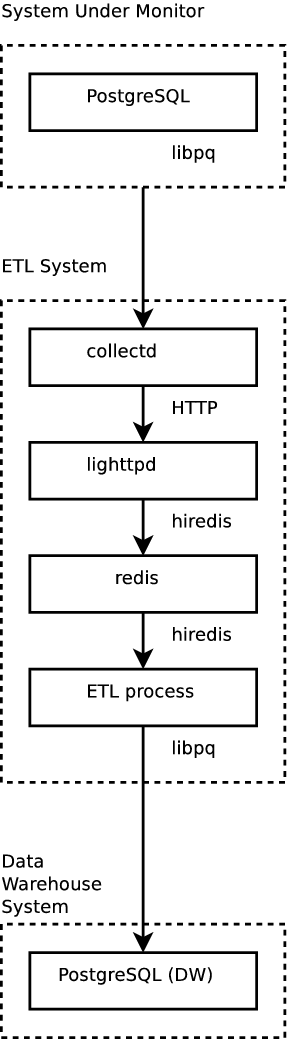
\includegraphics[scale=0.35]{a}
  \end{center}
  \caption{YAMS Architecture}
  \label{architecture}
\end{figure}

\subsection{Collecting statistics}

collectd offers the ability to monitor many aspects of a system without
restricting the system to use a specific data store or visualization interface.
It offers many system statistic collection plugins for areas including
processor, memory, storage, network, and a query interface for PostgreSQL.
There are also several output plugins that can be taken advantage of, in
particular we decided to take advantage of the \textit{write\_http}
plugin\footnote{\url{http://collectd.org/wiki/index.php/Plugin:Write_HTTP}},
which submits statistics using HTTP POST requests as JSON objects.

Yet collectd still needed some modifications to fit our specific needs.  In
order to gather individual table and index statistics we needed to make a
couple of changes collectd. First we needed to be able to annotate metadata to
the metrics that collectd gathers.  The collectd project has accepted a patch
to do that and has released it since version 5.2.  The second change we need is
to be able to create metadata identifying the database, schema, table and index
to the postgresql plugin.  We have patch proposed to do this and have submitted
it back to the collectd
community.\footnote{\url{http://mailman.verplant.org/pipermail/collectd/2013-May/005778.html}} 

We recognize that an alternative to annotating the database, schema, table and
index names to the JSON object as metadata is to take advantage of the
\texttt{type\_instance} field in the \texttt{value\_list} data structure in
collectd.  The issue here is that the \texttt{type\_instance} character array
is defined to only hold up to 64 characters.  PostgreSQL allows database,
schema, table and index names to be up to 255 characters each.  This means
that the \texttt{type\_instance} character array needs to be at least 1020
characters long.

\subsection{Database schema design}

PostgreSQL's table inheritance is used to implement a basic horizontal
partitioning of the data.  The intent is to keep the data size in the database
manageable and faster to query.  The parent table DDL (data definition
language) for all of the child tables is defined in
Figure~\ref{fig:parent_ddl}.

\begin{figure*}
  \lstset{language=sql}
  \begin{lstlisting}
CREATE TABLE value_list (
    time TIMESTAMP WITH TIME ZONE NOT NULL,
    interval INTEGER NOT NULL,
    host VARCHAR(64) NOT NULL,
    plugin VARCHAR(64) NOT NULL,
    plugin_instance VARCHAR(64),
    type VARCHAR(64) NOT NULL,
    type_instance VARCHAR(64),
    dsnames VARCHAR(512)[] NOT NULL,
    dstypes VARCHAR(8)[] NOT NULL,
    values NUMERIC[] NOT NULL,
    meta HSTORE NOT NULL DEFAULT ''
);
  \end{lstlisting}
  \caption{DDL for parent table}
  \label{fig:parent_ddl}
\end{figure*}

The maximum values for each column are defined based on the maximum possible
value that collectd can provide.  The data is partitioned by inheriting the
\textbf{value\_list} table for each day's worth of data per plugin used.  For
example, a \textit{cpu} plugin-partitioned tables on January 31, 2012 would be
created as shown in Figure~\ref{fig:cpu_ddl}.

\begin{figure*}
  \lstset{language=sql}
  \begin{lstlisting}
CREATE TABLE vl_cpu_20130231 (
    CHECK (time >= '2013-01-31 00:00:00'::TIMESTAMP AT TIME ZONE 'UTC'
       AND time < '2013-02-01 00:00:00'::TIMESTAMP AT TIME ZONE 'UTC'),
    CHECK (plugin = 'cpu')
) INHERITS (value_list);
  \end{lstlisting}
  \caption{DDL for cpu plugin child table}
  \label{fig:cpu_ddl}
\end{figure*}

Additional considerations were taken in the partitioning scheme for the
\textit{postgresql} plugin.  With approximately 50,000 tables in the redesigned
platform there are 900,000 data points gathered from all of the table
statistics tables per sample interval.  Similarly, with approximately 200,000
indexes there are 1,000,000 data points gathered from all of the index
statistics tables.  At five minute sample intervals this total nears
550,000,000 data points inserted into the database over the course of a day.
To help manage this the collectd postgresql plugin tables are further
partitioned by type, in this case separate tables will be created for table
statistics and index statistics.  The table definition for the
\textit{postgresql} plugin is defined as shown in
Figure~\ref{fig:postgresql_ddl} for the table statistics.

\begin{figure*}
  \lstset{language=sql}
  \begin{lstlisting}
CREATE TABLE vl_postgresql_20130131_table_stats (
    CHECK (time >= '2013-01-31 00:00:00'::TIMESTAMP AT TIME ZONE 'UTC'
       AND time < '2013-02-01 00:00:00'::TIMESTAMP AT TIME ZONE 'UTC'),
    CHECK (plugin = 'postgresql'),
    CHECK (type = 'table_stats')
) INHERITS (value_list);
  \end{lstlisting}
  \caption{DDL for postgresql plugin child table}
  \label{fig:postgresql_ddl}
\end{figure*}

PostgreSQL's \textit{constraint exclusion} is a query optimization technique
that leverages the \textit{CHECK} constraints to determine which child tables
are accessed when the parent table is queried.  Querying the parent
\textit{value\_list} table and specifying \textit{time} and \textit{plugin}
will direct the query planner to the appropriate tables.

\section{Gathering PostgreSQL statistics}

Here are is a short example of how table statistics are retrieved from
PostgresSQL.\footnote{These examples have been reformatted for easier reading.
See full examples in the source code repository.}  The collectd
\textit{postgresql} documentation
\footnote{\url{http://collectd.org/documentation/manpages/collectd.conf.5.shtml#plugin_postgresql}}
has complete details on how this plugin is used.  Only differences introduced
by our patches are explained in this paper.

Table statistics can be queried from the \textit{pg\_stats\_all\_tables},
\textit{pg\_statsio\_all\_tables} or \textit{pg\_class} tables.  The
\textit{collectd.conf} example shown in Figure~\ref{fig:collectd_conf}
describes how to collect some of the table statistics in PostgreSQL.

\begin{figure*}
  \lstset{language=xml}
  \begin{lstlisting}
<Plugin postgresql>
	<Query stat_table>
		Statement "SELECT schemaname, relname, seq_scan, seq_tup_read
		           FROM pg_stat_all_tables;"
		<Result>
			Type table_stats
			InstancePrefix "table_stats
			InstancesFrom "relname" "schemaname"
			ValuesFrom "seq_scan"
			SchemaNameFrom "schemaname"
			TableNameFrom "relname"
		</Result>
	</Query>
	<Database pgdatabase>
		Host "pghost"
		User "pguser"
		Query stat_table
	</Database>
</Plugin>
  \end{lstlisting}
  \caption{collectd.conf example}
  \label{fig:collectd_conf}
\end{figure*}

The \textit{SchemaNameFrom} and \textit{TableNameFrom} fields tells the
\textit{postgresql} plugin to create a metadata field named \textit{schema} and
\textit{table}, respectively, and to set the value to the data returned from
the \textit{schemaname} and \textit{relname} columns, respectively, from the
query.  The database name does not necessarily need to be specified in the
query since we can only collect table stats from a single database at a time.
In this case the plugin will use the database name set in the <Database> block
and set the metadata \textit{database} to this value.\footnote{As of collectd
v5.2 there is a parameter can be set to override the value set in the
<Database> block.}  Yet there may be a case where we want to set the database
name as part of the query.  A column can be specified for the database name
with the \textit{DatabaseNameFrom} field, similarly when collecting index
statistics the \textit{IndexNameFrom} field can be specified to create metadata
with the index name.

Note that the \textit{Type} of \textit{table\_stats} is a custom collectd data
type.\footnote{http://collectd.org/documentation/manpages/types.db.5.shtml}  It
is as defined as shown in Figure~\ref{fig:custom_type}.  While it isn't
required to define a custom data type, creating a custom type in this way makes
collectd build an array of metrics, in this case a single collectd record that
contains values from both \textit{seq\_scan} and \textit{seq\_tup\_read}.

\begin{figure*}
  \begin{lstlisting}
table_stats seq_scan:COUNTER:0:U seq_tup_read:COUNTER:0:U
  \end{lstlisting}
  \caption{Custom collectd data type}
  \label{fig:custom_type}
\end{figure*}

By taking advantage of the database array data type only a single insert is
needed to load all the metrics queried per table into the database.

\section{Performance and sizing characterization}

Is it even possible to implement a solution like this?

Tuning of filesystems and storage subsystems is outside the scope of the this
paper.  We attempted to ensure the storage subsystem had enough capacity and
throughput to sustain collecting data from a 1 million table PostgreSQL
database.  These results are not meant to be interpreted as the best tuned
storage solution.  There are three areas that generated measurable amounts of
I/O on the data warehouse system when inserting collectd data: the PostgreSQL
transaction log, the collectd tablespace, and the PostgreSQL system catalog
tables.  A separate single spindle device is used for the pgdata device, which
includes the PostgreSQL system catalog tables and statistics file, and the
collectd tablespace.  The device supporting the pgdata directory peaks at about
4 I/O operations per second, while the collectd tablespace peaks at almost 60
I/O operations per second.  The PostgreSQL transaction log device needed
significant I/O operation performance in order to sustain a high level of
inserts into the data warehouse.  It was measured that about 250 writes per
second were sustained when processing approximately 8,000 items from Redis per
minute.  To simplify our proof of concept we used a 6 GB tmpfs volatile
filesystem in memory instead of utilizing more hard drives in the system.
We note that solid state storage would be more practical in a production
environment as high rates of I/O are far more important than storage capacity
for the PostgreSQL transaction log, but we did not have any available for this
work.

\begin{figure}[ht]
  \begin{center}
    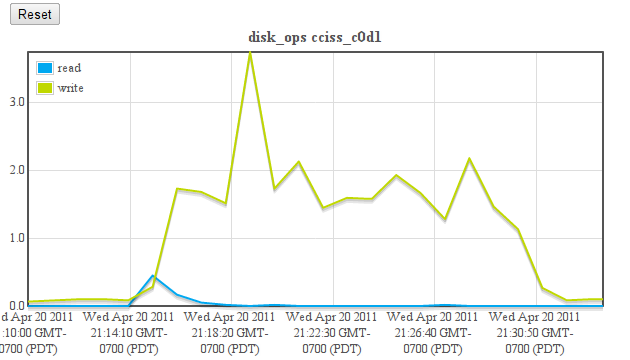
\includegraphics[scale=0.37]{etl-c6-disk-c0d1-iops}
  \end{center}
  \caption{Data Warehouse System pgdata Device During Data Processing}
  \label{etl-c6-c0d1}
\end{figure}

\begin{figure}[ht]
  \begin{center}
    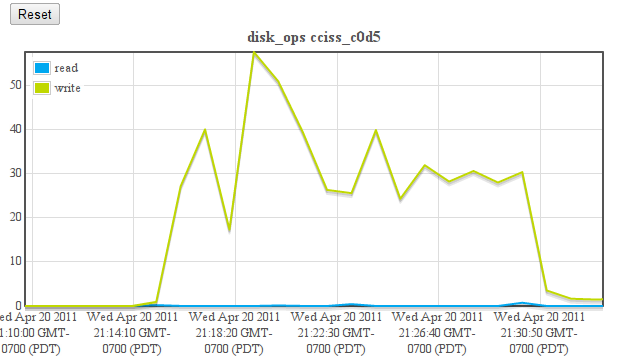
\includegraphics[scale=0.37]{etl-c6-disk-c0d5-iops}
  \end{center}
  \caption{Data Warehouse System collectd Tablespace Device During Data
           Processing}
  \label{etl-c6-c0d5}
\end{figure}

\section{Conclusions and Future Work}

From experience with the database systems at Emma we know that the performance
of the YAMS database system will be greatly affected because of the
partitioning scheme used.  The number of tables will affect the statistics
collection process in PostgreSQL.  When the number of tables and indexes
increases into the hundred of thousands, PostgreSQL's temporary statistics file
will need to place onto a high performance device such as a solid state device
or volatile memory.

This prototype is by no stretch of the imagination a light weight or
inexpensive solution.  Significant hardware resources for the data warehouse
system are required to handle large volumes of data.  The ETL system likely
needs at least 16 GB of memory to operate efficiently by avoiding swapping any
memory to disk.  The data warehouse system needs solid state storage, or many
spindles of hard disk drives, in order to support high insert rates.  Terabytes
of storage for storing data long term may be relatively inexpensive compared to
the I/O operations needed for the PostgreSQL transaction logs.  It may also be
prudent to have at least a dedicated 100 mbit network between the ETL system
and the data warehouse if a 1 gbit or faster network is not available.  With
the hardware used in this paper, we can only hope to achieve a sample interval
of 15 minutes for database statistics.  Note that other system statistics can
still be collected at more frequent intervals.

There may be further optimizations that can be done with collectd such that
data can be submitted to the ETL more quickly, perhaps by changing the size of
the buffer size for the HTTP POST request.  We also considered exploring
whether the \textit{write\_http} plugin in collectd should be modified to
submit data to the ETL asynchronously.  Similarly we considered modifying the C
FastCGI application could be altered to push data to Redis asynchronously.
Perhaps using compression may reduce the network bandwidth required when
sending JSON data across the network.

The graphs of system statistics used in this paper are screen shots taken from
a prototype Web user interface using the Flotr JavaScript Plotting
Library\footnote{\url{http://solutoire.com/flotr/}} built on a Pylons
Project\footnote{\url{http://pylonsproject.org/}} application.  The next steps
in building this monitoring system is to provide a more complete user interface
that will display common metrics such as processor, memory, network, and
storage utilization, as well as PostgreSQL database specific information such
as table and index bloat, vacuuming and analyze history, and table and index
utilization.  Other features such as authentication and authorization would
also be desired.

\section{Acknowledgements}

Many thanks to the following for donating resources to PostgreSQL,
which makes projects like this possible.  Emma, Inc. for letting us release the
start of our work as open source software and supporting our efforts with the
PostgreSQL global development community.  Sun Microsystems for the Sun Fire
T2000 server.  HP for two DL380 G5 servers and an MSA70 Modules Smart Array.
IBM for two Apple Power Mac G5 systems.  Hi5.com for four Dell PowerVault
storage devices.  Command Prompt for space in their co-location facility.

Also special thanks to my colleagues from the PostgreSQL Global Development
Community and Emma Gabrielle Roth, Selena Deckelmann and Marc Powell for their
support.

\bibliographystyle{alpha}
\bibliography{bibliography}

\section*{Appendix A}

These figures represent the individual processor utilization of each core on
the ETL system during the time collectd retrieved PostgreSQL table statistics
and push them to the ETL system.

\begin{figure}[ht]
  \begin{center}
    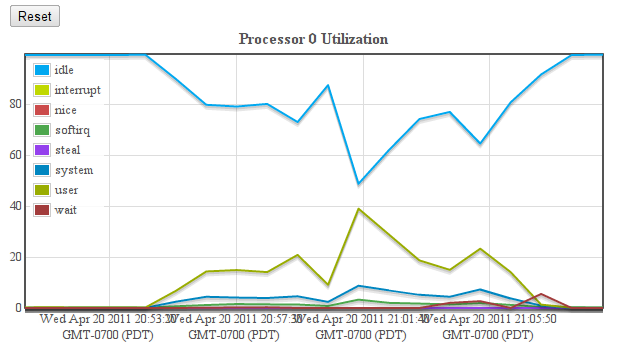
\includegraphics[scale=0.37]{collectd-c10-cpu-00}
  \end{center}
  \caption{ETL System Processor 0}
  \label{collectd-c10-cpu00}
\end{figure}

\begin{figure}[ht]
  \begin{center}
    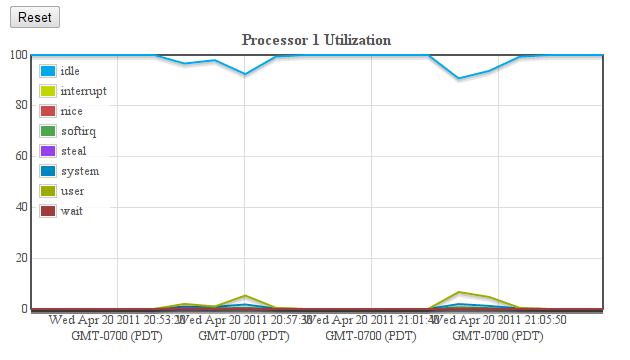
\includegraphics[scale=0.37]{collectd-c10-cpu-01}
  \end{center}
  \caption{ETL System Processor 1}
\end{figure}

\begin{figure}[ht]
  \begin{center}
    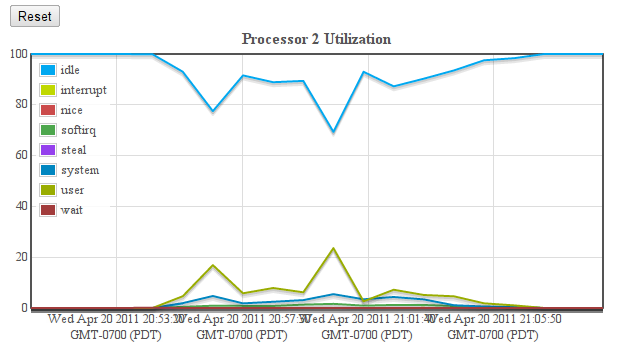
\includegraphics[scale=0.37]{collectd-c10-cpu-02}
  \end{center}
  \caption{ETL System Processor 2}
\end{figure}

\begin{figure}[ht]
  \begin{center}
    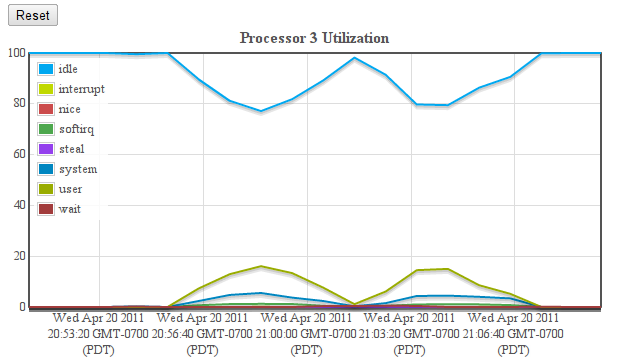
\includegraphics[scale=0.37]{collectd-c10-cpu-03}
  \end{center}
  \caption{ETL System Processor 3}
\end{figure}

\begin{figure}[ht]
  \begin{center}
    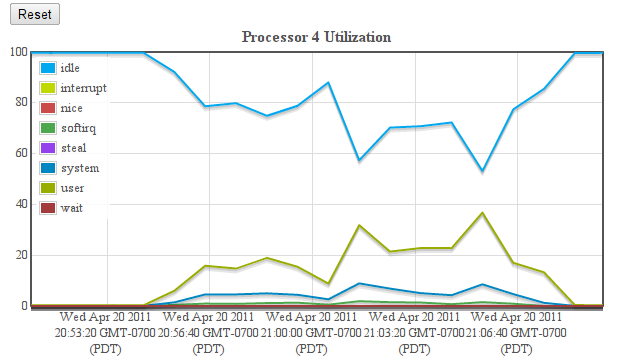
\includegraphics[scale=0.37]{collectd-c10-cpu-04}
  \end{center}
  \caption{ETL System Processor 4}
\end{figure}

\begin{figure}[ht]
  \begin{center}
    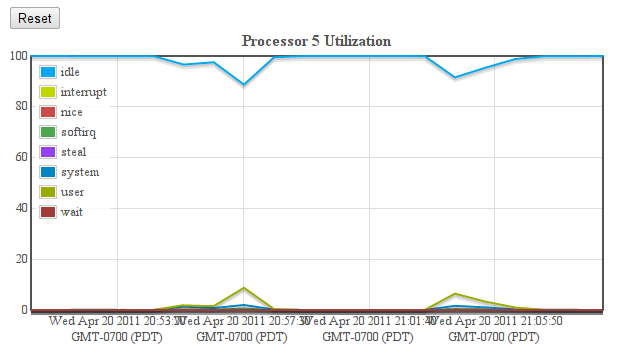
\includegraphics[scale=0.37]{collectd-c10-cpu-05}
  \end{center}
  \caption{ETL System Processor 5}
\end{figure}

\begin{figure}[ht]
  \begin{center}
    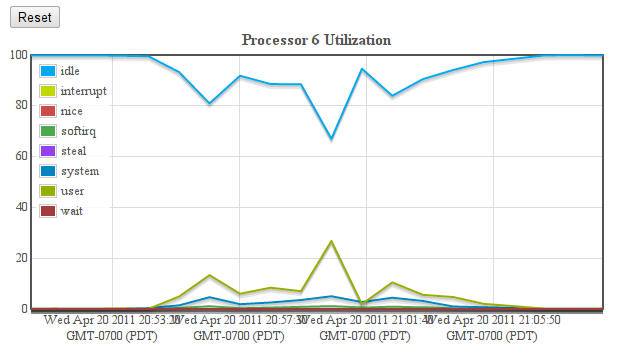
\includegraphics[scale=0.37]{collectd-c10-cpu-06}
  \end{center}
  \caption{ETL System Processor 6}
\end{figure}

\begin{figure}[ht]
  \begin{center}
    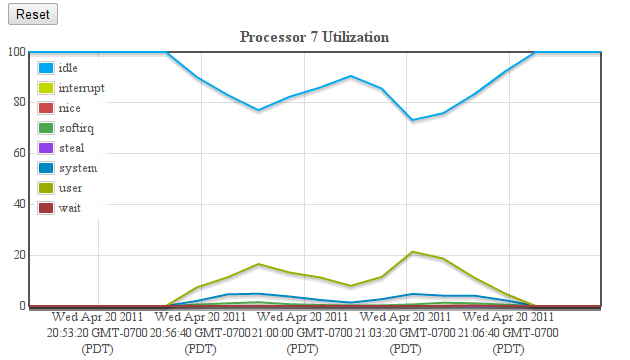
\includegraphics[scale=0.37]{collectd-c10-cpu-07}
  \end{center}
  \caption{ETL System Processor 7}
  \label{collectd-c10-cpu07}
\end{figure}

\section*{Appendix B}

These figures represent the individual processor utilization of each core on
the ETL system during the time the ETL system processed the collectd data and
inserted the data into the data warehouse.

\begin{figure}[ht]
  \begin{center}
    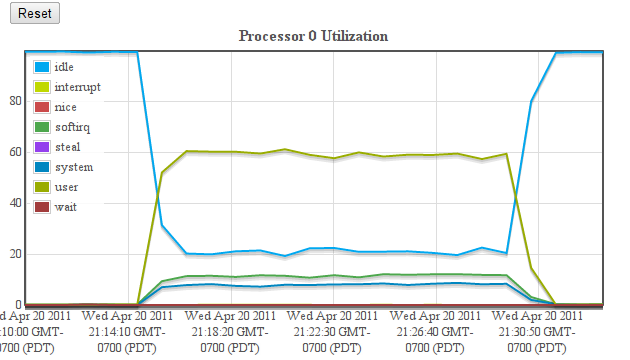
\includegraphics[scale=0.37]{etl-c10-cpu-00}
  \end{center}
  \caption{ETL System Processor 0}
  \label{etl-c10-cpu00}
\end{figure}

\begin{figure}[ht]
  \begin{center}
    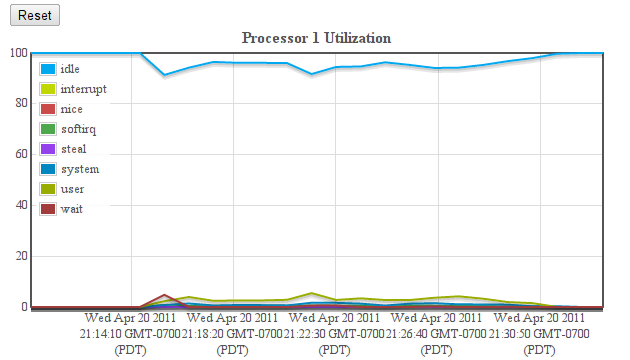
\includegraphics[scale=0.37]{etl-c10-cpu-01}
  \end{center}
  \caption{ETL System Processor 1}
\end{figure}

\begin{figure}[ht]
  \begin{center}
    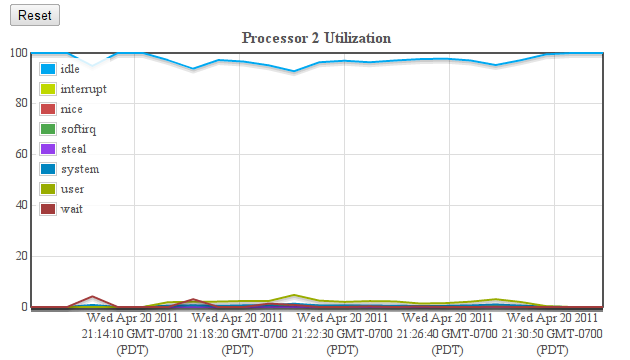
\includegraphics[scale=0.37]{etl-c10-cpu-02}
  \end{center}
  \caption{ETL System Processor 2}
\end{figure}

\begin{figure}[ht]
  \begin{center}
    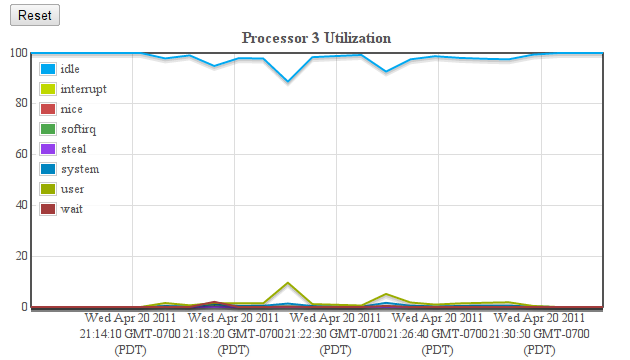
\includegraphics[scale=0.37]{etl-c10-cpu-03}
  \end{center}
  \caption{ETL System Processor 3}
\end{figure}

\begin{figure}[ht]
  \begin{center}
    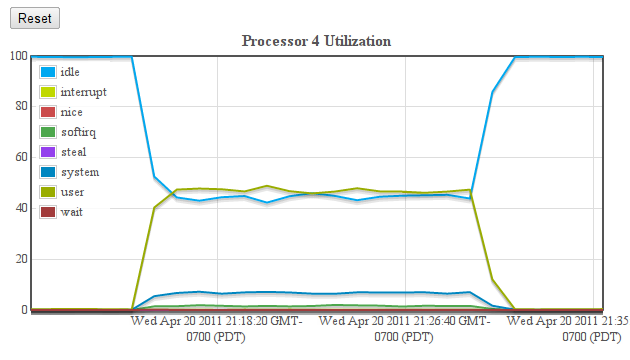
\includegraphics[scale=0.37]{etl-c10-cpu-04}
  \end{center}
  \caption{ETL System Processor 4}
\end{figure}

\begin{figure}[ht]
  \begin{center}
    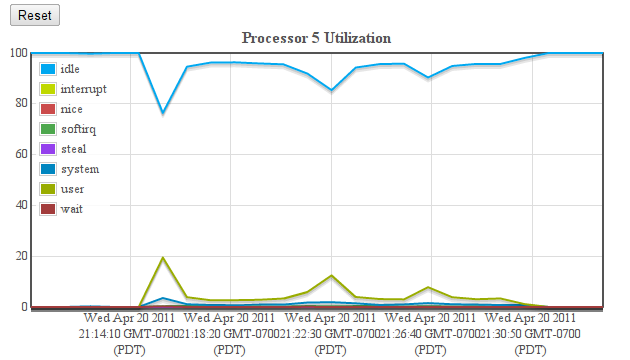
\includegraphics[scale=0.37]{etl-c10-cpu-05}
  \end{center}
  \caption{ETL System Processor 5}
\end{figure}

\begin{figure}[ht]
  \begin{center}
    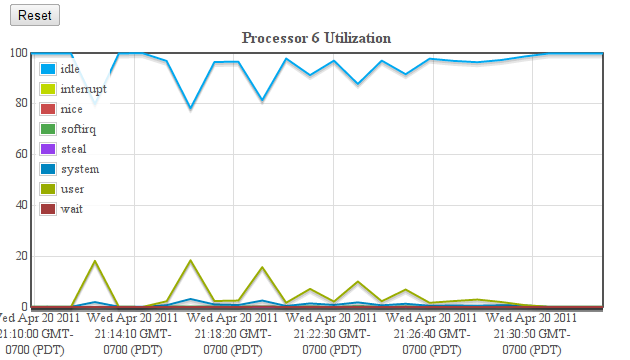
\includegraphics[scale=0.37]{etl-c10-cpu-06}
  \end{center}
  \caption{ETL System Processor 6}
\end{figure}

\begin{figure}[ht]
  \begin{center}
    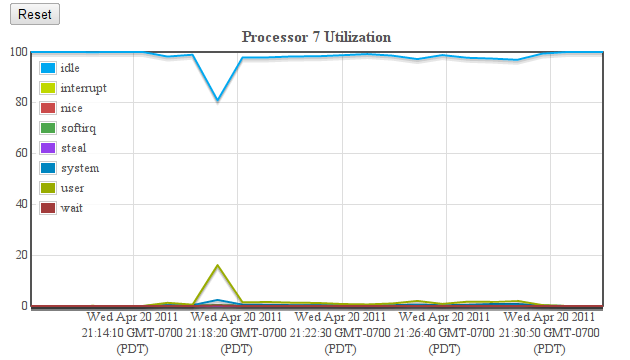
\includegraphics[scale=0.37]{etl-c10-cpu-07}
  \end{center}
  \caption{ETL System Processor 7}
  \label{etl-c10-cpu07}
\end{figure}

\section*{Appendix C}

These figures represent the individual processor utilization of each core on
the data warehouse system during the time the ETL system processed the collectd
data and inserted the data into the data warehouse.

\begin{figure}[ht]
  \begin{center}
    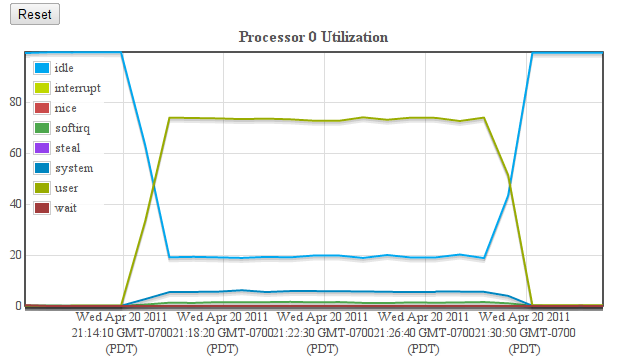
\includegraphics[scale=0.37]{etl-c6-cpu-00}
  \end{center}
  \caption{Data Warehouse System Processor 0}
  \label{etl-c6-cpu00}
\end{figure}

\begin{figure}[ht]
  \begin{center}
    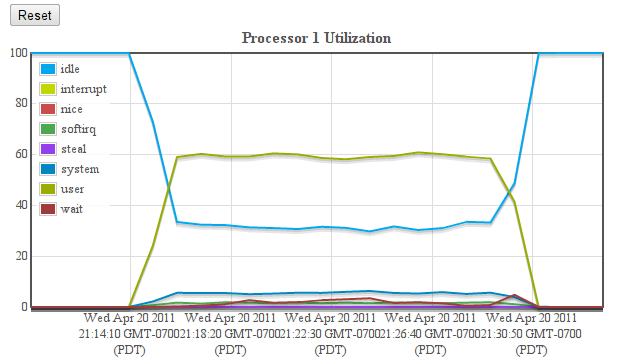
\includegraphics[scale=0.37]{etl-c6-cpu-01}
  \end{center}
  \caption{Data Warehouse System Processor 1}
\end{figure}

\begin{figure}[ht]
  \begin{center}
    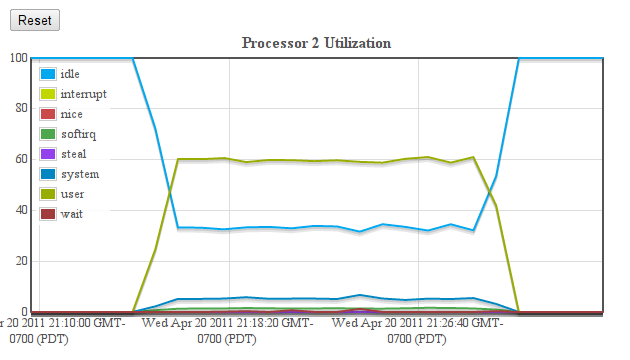
\includegraphics[scale=0.37]{etl-c6-cpu-02}
  \end{center}
  \caption{Data Warehouse System Processor 2}
\end{figure}

\begin{figure}[ht]
  \begin{center}
    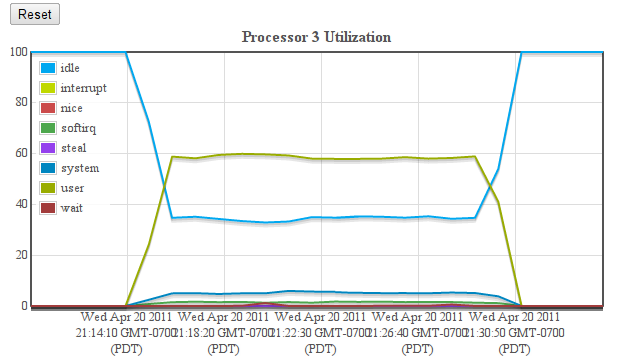
\includegraphics[scale=0.37]{etl-c6-cpu-03}
  \end{center}
  \caption{Data Warehouse System Processor 3}
\end{figure}

\begin{figure}[ht]
  \begin{center}
    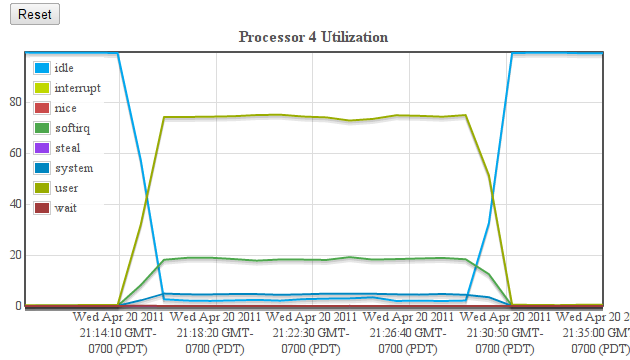
\includegraphics[scale=0.37]{etl-c6-cpu-04}
  \end{center}
  \caption{Data Warehouse System Processor 4}
\end{figure}

\begin{figure}[ht]
  \begin{center}
    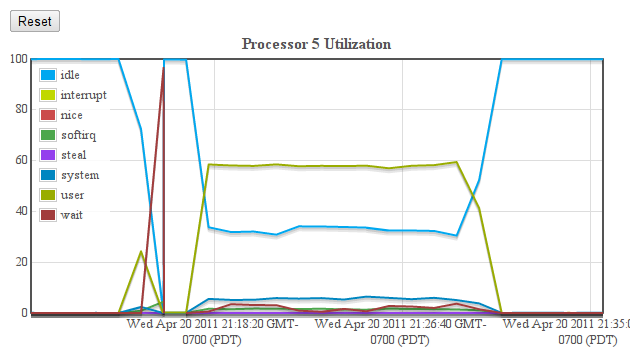
\includegraphics[scale=0.37]{etl-c6-cpu-05}
  \end{center}
  \caption{Data Warehouse System Processor 5}
\end{figure}

\begin{figure}[ht]
  \begin{center}
    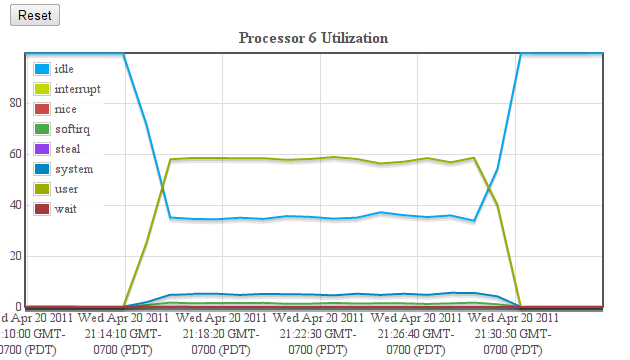
\includegraphics[scale=0.37]{etl-c6-cpu-06}
  \end{center}
  \caption{Data Warehouse System Processor 6}
\end{figure}

\begin{figure}[ht]
  \begin{center}
    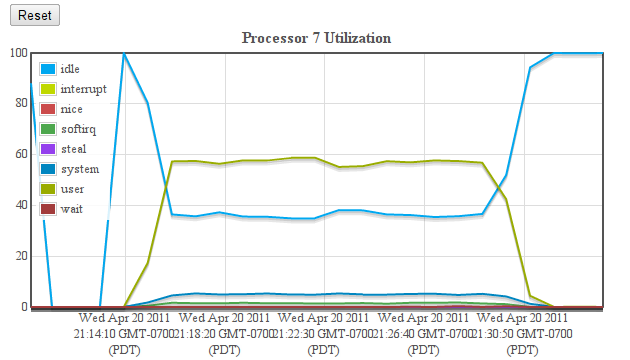
\includegraphics[scale=0.37]{etl-c6-cpu-07}
  \end{center}
  \caption{Data Warehouse System Processor 7}
  \label{etl-c6-cpu07}
\end{figure}

\end{document}
